\documentclass[11pt,a4paper]{article}
\usepackage[T1]{fontenc}
\usepackage[utf8]{inputenc}
\usepackage[provide=*,italian]{babel}
\usepackage{lmodern,microtype}
\usepackage{geometry}
\geometry{margin=2.5cm}
\usepackage{amsmath,amssymb,amsthm,mathtools}
\usepackage{booktabs,array,longtable}
\usepackage{xcolor,enumitem}
\usepackage{tikz}
\usetikzlibrary{arrows.meta,positioning,calc,fit}
\usepackage[most]{tcolorbox}
\usepackage{hyperref,fancyhdr}

\definecolor{sapienzared}{RGB}{130,0,36}
\definecolor{softred}{RGB}{249,241,243}
\definecolor{softblue}{RGB}{239,246,252}
\definecolor{softgray}{RGB}{245,245,245}
\hypersetup{colorlinks=true,linkcolor=sapienzared,urlcolor=sapienzared,
pdftitle={Introduzione all'ottimizzazione su reti},pdfauthor={Giampaolo Liuzzi}}

\pagestyle{fancy}
\fancyhf{}
\fancyhead[L]{\small Ottimizzazione su Reti}
\fancyhead[R]{\small Capitolo 1}
\fancyfoot[C]{\thepage}
\renewcommand{\headrulewidth}{0.4pt}

\newtcolorbox{learningbox}{colback=softred,colframe=sapienzared,
title=Obiettivi di apprendimento,fonttitle=\bfseries,boxrule=0.8pt,arc=1.5mm}
\newtcolorbox{examplebox}[1]{colback=softblue,colframe=blue!55!black,
title=#1,fonttitle=\bfseries,boxrule=0.7pt,arc=1.5mm}
\newtcolorbox{notationbox}{colback=softgray,colframe=black!55,
title=Registro delle notazioni,fonttitle=\bfseries,boxrule=0.7pt,arc=1.5mm}
\newtcolorbox{keybox}{colback=softred,colframe=sapienzared,boxrule=0.8pt,arc=1.5mm}

\newcommand{\V}{\mathcal{V}}
\newcommand{\E}{\mathcal{E}}
\newcommand{\R}{\mathbb{R}}

\begin{document}
\hypersetup{pageanchor=false}
\begin{titlepage}
\centering
\vspace*{1.6cm}
{\color{sapienzared}\rule{\textwidth}{1.2pt}}\\[1.1cm]
{\Large Ottimizzazione su Reti}\\[0.35cm]
{\huge\bfseries Capitolo 1}\\[0.45cm]
{\LARGE\bfseries Introduzione all'ottimizzazione su reti}\\[1.1cm]
{\color{sapienzared}\rule{0.72\textwidth}{0.8pt}}\\[1.1cm]
{\large Corso di Laurea Magistrale in Ingegneria Gestionale}\\[0.25cm]
{\large Sapienza Università di Roma}\\[1.2cm]
{\large Giampaolo Liuzzi}\\[0.25cm]
{\normalsize Dipartimento di Ingegneria Informatica, Automatica e Gestionale}\\[2cm]
\vfill
{\small Versione preliminare per uso didattico}
\end{titlepage}

\hypersetup{pageanchor=true}
\pagenumbering{roman}
\tableofcontents
\newpage
\pagenumbering{arabic}

\begin{learningbox}
Al termine del capitolo lo studente dovrebbe essere in grado di:
\begin{itemize}[nosep]
\item riconoscere situazioni decisionali rappresentabili mediante grafi;
\item distinguere tra rete, modello matematico, algoritmo e soluzione;
\item spiegare perché la struttura di rete consente algoritmi specializzati;
\item identificare dati, decisioni, vincoli e obiettivo in un'applicazione;
\item descrivere il percorso logico del corso;
\item usare correttamente la notazione introduttiva che sarà mantenuta nei capitoli successivi.
\end{itemize}
\end{learningbox}

\section{Che cos'è l'ottimizzazione su reti}

Molti sistemi reali sono costituiti da oggetti collegati tra loro: città connesse da strade, depositi e clienti collegati da rotte di distribuzione, router connessi da canali di comunicazione, attività legate da relazioni di precedenza. Un grafo offre una rappresentazione naturale di questi sistemi; l'ottimizzazione su reti studia come prendere decisioni efficienti sfruttando tale rappresentazione.

In termini generali, un problema di ottimizzazione richiede di scegliere valori per alcune \emph{variabili decisionali}, rispettando un insieme di \emph{vincoli}, in modo da rendere minima o massima una \emph{funzione obiettivo}. Nei problemi su rete, variabili e vincoli possiedono una struttura strettamente legata a nodi e archi del grafo.

\begin{keybox}
La rete non è ancora il problema di ottimizzazione. Essa descrive la struttura delle relazioni. Per ottenere un modello occorre specificare dati, decisioni ammissibili, vincoli e criterio di scelta.
\end{keybox}

\subsection{Quattro livelli da non confondere}

\begin{center}
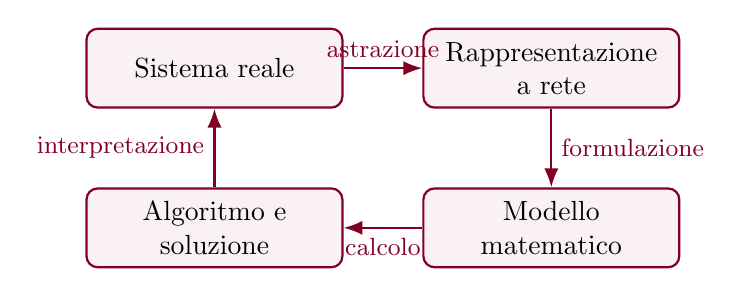
\begin{tikzpicture}[
box/.style={draw=sapienzared,thick,rounded corners,fill=softred,
minimum width=3.25cm,minimum height=1cm,align=center},
arr/.style={-{Latex[length=2.4mm]},thick,sapienzared}
]
\node[box] (reale) {Sistema reale};
\node[box,right=1.0cm of reale] (rete) {Rappresentazione\\a rete};
\node[box,below=1.0cm of rete] (modello) {Modello\\matematico};
\node[box,left=1.0cm of modello] (soluzione) {Algoritmo e\\soluzione};
\draw[arr] (reale) -- node[above,font=\small]{astrazione} (rete);
\draw[arr] (rete) -- node[right,font=\small]{formulazione} (modello);
\draw[arr] (modello) -- node[below,font=\small]{calcolo} (soluzione);
\draw[arr] (soluzione) -- node[left,font=\small]{interpretazione} (reale);
\end{tikzpicture}
\end{center}

\begin{enumerate}
\item Il \textbf{sistema reale} contiene oggetti, relazioni e decisioni possibili.
\item La \textbf{rete} conserva gli elementi rilevanti attraverso nodi e archi.
\item Il \textbf{modello matematico} introduce variabili, parametri, vincoli e obiettivo.
\item L'\textbf{algoritmo} produce una soluzione che deve essere interpretata nel sistema reale.
\end{enumerate}

\section{Perché usare i grafi}

La rappresentazione mediante grafi è utile quando le relazioni tra gli oggetti sono importanti quanto gli oggetti stessi. Essa consente di:
\begin{itemize}
\item visualizzare la struttura del problema;
\item distinguere proprietà topologiche e dati quantitativi;
\item riconoscere problemi già studiati;
\item applicare risultati teorici specifici;
\item utilizzare algoritmi che sfruttano la sparsità e la struttura combinatoria;
\item interpretare la soluzione come cammino, albero, flusso, taglio o sequenza di attività.
\end{itemize}

\subsection{Algoritmi generali e algoritmi specializzati}

Molti problemi su rete possono essere formulati come problemi di programmazione lineare. È quindi possibile, almeno in linea di principio, utilizzare un metodo generale. La particolare struttura della matrice dei vincoli permette però di costruire algoritmi più trasparenti ed efficienti.

Nel corso incontreremo entrambi i punti di vista:
\begin{itemize}
\item il \emph{flusso a costo minimo} come modello generale di programmazione lineare su rete;
\item il \emph{simplesso su reti} come specializzazione del simplesso;
\item massimo flusso, cammino minimo e altri problemi come casi particolari;
\item algoritmi dedicati, quali Ford--Fulkerson, Bellman--Ford e Dijkstra.
\end{itemize}

Questa doppia lettura consente di capire non solo \emph{come} applicare un algoritmo, ma anche \emph{perché} esso è corretto e quali informazioni certificano l'ottimalità.

\section{Esempi di problemi rappresentabili mediante reti}

\subsection{Confini geografici}

Consideriamo le regioni italiane e la relazione ``confina con''. Ogni regione può essere rappresentata da un nodo e ogni coppia di regioni confinanti da uno spigolo. La relazione è simmetrica: se la regione $A$ confina con $B$, anche $B$ confina con $A$. Il grafo è quindi non orientato.

Questo semplice esempio introduce due scelte essenziali:
\begin{enumerate}[label=(\alph*)]
\item quali oggetti devono diventare nodi;
\item quali relazioni devono diventare archi o spigoli.
\end{enumerate}
Non è ancora presente un obiettivo di ottimizzazione, ma la struttura ottenuta permette già di studiare connessione, adiacenza, cammini e componenti connesse.

\subsection{Distribuzione e trasporto}

Una società deve inviare prodotti da alcuni depositi a un insieme di clienti, utilizzando centri intermedi e collegamenti con capacità limitata. I nodi rappresentano depositi, clienti e centri di transito; gli archi rappresentano i collegamenti utilizzabili. A ogni arco possono essere associati costo e capacità.

Le decisioni sono le quantità inviate sui collegamenti. I vincoli esprimono la conservazione del flusso e il rispetto delle capacità; l'obiettivo può essere la minimizzazione del costo complessivo.

\subsection{Instradamento in una rete di telecomunicazione}

Un provider deve trasferire traffico dai data center ai punti di accesso, passando eventualmente attraverso router intermedi. Ogni link ha una capacità massima e un costo per unità di banda. Il problema consiste nel soddisfare tutte le richieste minimizzando il costo operativo.

Questo esempio sarà ripreso nei capitoli sul flusso a costo minimo e sul simplesso su reti.

\subsection{Scelta di percorsi}

In una rete stradale, i nodi possono rappresentare incroci o città e gli archi tratti percorribili. A ogni arco è associato un costo: distanza, tempo, pedaggio o una loro combinazione. La decisione consiste nella scelta di un cammino; l'obiettivo è minimizzarne il costo.

Il significato di ``cammino migliore'' dipende dunque dai dati e dall'obiettivo, non dalla sola struttura del grafo.

\subsection{Capacità di una rete}

In una rete con una sorgente e una destinazione può essere necessario determinare la quantità massima trasferibile. Le capacità degli archi limitano il flusso; la soluzione è collegata a un taglio che separa la sorgente dalla destinazione. Questo conduce ai problemi di massimo flusso e minimo taglio.

\subsection{Pianificazione di un progetto}

Consideriamo l'organizzazione di un congresso scientifico. Tra le attività figurano:
\begin{itemize}[nosep]
\item definizione del tema e degli obiettivi;
\item costituzione del comitato scientifico;
\item scelta della sede e definizione del budget;
\item realizzazione del sito e pubblicazione della call for papers;
\item revisione dei contributi e preparazione del programma;
\item comunicazione, allestimento e logistica.
\end{itemize}
Le attività non possono essere eseguite in un ordine arbitrario. Le precedenze formano un grafo orientato aciclico; durate e relazioni consentono di calcolare la durata minima del progetto e di individuare le attività critiche mediante il Critical Path Method.

\section{Dall'applicazione al modello}

Prima di scegliere un algoritmo conviene rispondere sistematicamente ad alcune domande.

\begin{longtable}{>{\bfseries}p{3.3cm}p{10.7cm}}
\toprule
Elemento & Domanda guida\\
\midrule
Nodi & Quali oggetti, luoghi, eventi o stati devono essere rappresentati?\\
Archi & Quali relazioni o transizioni sono ammesse? Sono orientate?\\
Dati & Quali costi, capacità, durate, offerte o domande sono noti?\\
Variabili & Quali quantità o scelte devono essere determinate?\\
Vincoli & Quali bilanci, precedenze o limiti devono essere rispettati?\\
Obiettivo & Che cosa significa ``migliore'': costo minimo, flusso massimo, durata minima?\\
Soluzione & Come deve essere interpretato il risultato nel problema originario?\\
\bottomrule
\end{longtable}

\begin{examplebox}{Mini-esempio: consegna tra due città}
Una merce deve essere inviata dalla città $s$ alla città $t$. I collegamenti disponibili formano un grafo orientato e ogni arco ha un tempo di percorrenza. Se occorre inviare un solo mezzo, il problema è naturalmente un cammino minimo. Se occorre trasferire grandi quantità e ogni collegamento ha una capacità, il modello può invece diventare un problema di flusso. Lo stesso grafo può dunque sostenere modelli differenti.
\end{examplebox}

\section{Il percorso del corso}

Il corso adotta il flusso a costo minimo come modello centrale. Da esso vengono ricavate formulazioni di altri problemi, che saranno poi risolti anche mediante algoritmi specializzati.

\begin{center}
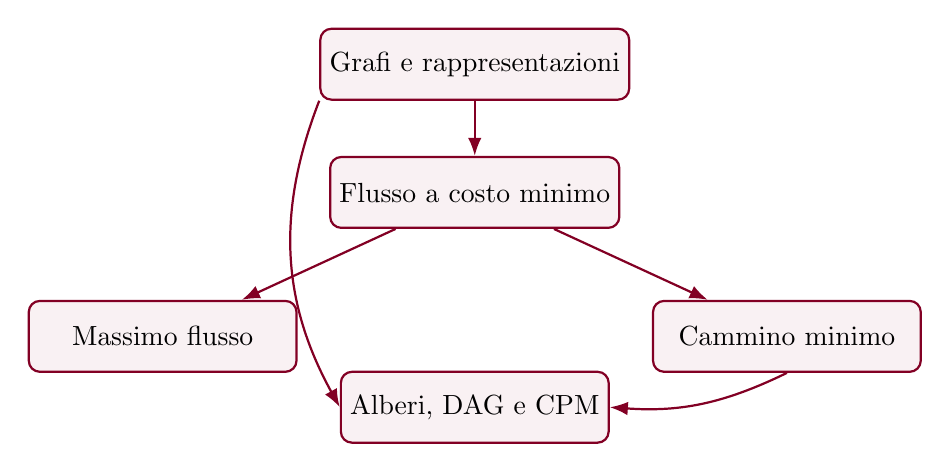
\begin{tikzpicture}[
box/.style={draw=sapienzared,thick,rounded corners,fill=softred,
minimum width=3.4cm,minimum height=9mm,align=center},
arr/.style={-{Latex[length=2.3mm]},thick,sapienzared}
]
\node[box] (grafi) {Grafi e rappresentazioni};
\node[box,below=7mm of grafi] (mcf) {Flusso a costo minimo};
\node[box,below left=9mm and 4mm of mcf] (max) {Massimo flusso};
\node[box,below right=9mm and 4mm of mcf] (sp) {Cammino minimo};
\node[box,below=18mm of mcf] (proj) {Alberi, DAG e CPM};
\draw[arr] (grafi) -- (mcf);
\draw[arr] (mcf) -- (max);
\draw[arr] (mcf) -- (sp);
\draw[arr] (grafi.south west) to[bend right=25] (proj.west);
\draw[arr] (sp.south) to[bend left=15] (proj.east);
\end{tikzpicture}
\end{center}

La sequenza concettuale è:
\begin{enumerate}
\item linguaggio dei grafi e rappresentazioni;
\item reti di flusso e matrice di incidenza;
\item flusso a costo minimo e simplesso su reti;
\item massimo flusso, minimo taglio e Ford--Fulkerson;
\item cammini minimi su DAG, Bellman--Ford e Dijkstra;
\item alberi ricoprenti e pianificazione di progetti mediante CPM.
\end{enumerate}

\section{Il ruolo degli strumenti computazionali}

Gli algoritmi saranno studiati sia manualmente, per comprenderne struttura e correttezza, sia mediante Python e NetworkX. Il software non sostituisce la modellazione: una funzione può restituire un risultato numericamente corretto per il grafo fornito, ma non può stabilire se quel grafo rappresenti correttamente il problema reale.

Il laboratorio computazionale seguirà quattro principi:
\begin{enumerate}
\item costruire e controllare l'istanza;
\item implementare una versione didattica dell'algoritmo;
\item confrontarla con la funzione di libreria;
\item verificare e interpretare la soluzione.
\end{enumerate}

\section{Registro delle notazioni e delle convenzioni}

\begin{notationbox}
\begin{center}
\begin{tabular}{>{$}l<{$}p{9.8cm}}
\toprule
G=(\V,\E) & grafo, con insieme dei nodi $\V$ e insieme degli archi o spigoli $\E$;\\
n=|\V| & numero dei nodi;\\
m=|\E| & numero degli archi o spigoli;\\
i,j,v & indici o nomi di nodi;\\
(i,j) & arco orientato dal nodo $i$ al nodo $j$;\\
\{i,j\} & spigolo non orientato tra $i$ e $j$, quando è utile distinguere esplicitamente i due casi;\\
c_{ij} & costo associato all'arco $(i,j)$;\\
x_{ij} & quantità decisionale associata all'arco $(i,j)$, quando applicabile.\\
\bottomrule
\end{tabular}
\end{center}
\end{notationbox}

Le notazioni $\delta^+(i)$, $\delta^-(i)$, la matrice di incidenza $A$ e il vettore dei bilanci $b$ saranno introdotti formalmente nei Capitoli 2--4. La convenzione già fissata per le reti di flusso sarà:
\[
\text{flusso entrante}-\text{flusso uscente}=b_i,
\qquad b_i>0\text{ per una domanda},\quad b_i<0\text{ per un'offerta}.
\]

\section{Esercizi introduttivi}

\subsection*{Esercizio 1.1 - Riconoscere nodi e archi}
Per ciascuno dei seguenti sistemi, proporre una scelta di nodi e archi e stabilire se il grafo debba essere orientato:
\begin{enumerate}[label=(\alph*)]
\item rete metropolitana;
\item rete di amicizie;
\item collegamenti tra pagine web;
\item precedenze tra insegnamenti di un corso di laurea;
\item rete di distribuzione di energia.
\end{enumerate}

\subsection*{Esercizio 1.2 - Uno stesso grafo, problemi diversi}
Considerare una rete stradale e descrivere almeno tre problemi di ottimizzazione differenti che possano essere formulati sullo stesso grafo. Per ciascuno indicare dati, variabili, vincoli e obiettivo.

\subsection*{Esercizio 1.3 - Organizzazione di un congresso}
Scegliere otto attività necessarie per organizzare un congresso scientifico e indicare le precedenze immediate. Discutere quali errori di modellazione potrebbero introdurre un ciclo nel grafo delle precedenze.

\subsection*{Esercizio 1.4 - Dal problema all'algoritmo}
Per ciascuna situazione, indicare la famiglia di problemi più plausibile tra cammino minimo, massimo flusso, flusso a costo minimo, albero ricoprente minimo e CPM:
\begin{enumerate}[label=(\alph*)]
\item collegare tutte le sedi aziendali minimizzando il costo della fibra;
\item determinare la massima quantità giornaliera trasportabile in un oleodotto;
\item soddisfare più clienti da più depositi minimizzando il costo;
\item trovare il percorso più rapido tra due città;
\item individuare le attività che determinano la durata di un progetto.
\end{enumerate}

\section{Sintesi del capitolo}

\begin{keybox}
\begin{itemize}[nosep]
\item Un grafo rappresenta oggetti e relazioni; un modello di ottimizzazione aggiunge dati, variabili, vincoli e obiettivo.
\item La struttura di rete permette interpretazioni chiare e algoritmi specializzati.
\item Lo stesso grafo può sostenere problemi decisionali differenti.
\item Una soluzione deve essere verificata matematicamente e interpretata nel sistema reale.
\item Il corso parte dal flusso a costo minimo e ricava massimo flusso e cammino minimo come casi particolari, prima di studiare algoritmi dedicati.
\item Notazione e convenzioni saranno mantenute uniformi in dispense, esercizi e notebook NetworkX.
\end{itemize}
\end{keybox}

\section*{Verso il capitolo successivo}
Il Capitolo 2 introdurrà formalmente grafi orientati e non orientati, cammini, cicli, connessione e principali rappresentazioni. Questi concetti costituiranno il linguaggio comune di tutti i modelli successivi.

\end{document}
